\chapter{Logistic Regression}

Now we turn away from regression to classification problems. Don't be confused by the name `logistic regression,' it's actually just named for the mathematical function and it's a common approach to classification.

\section{Binary Classification}
In classification problems, instead of our output being continuous, we expect it to fall into discrete classes. We'll start with the simplest case: binary classification. Here, we have our output variable $y \in \{0, 1\}$. Typically, we take $0$ as the negative class and $1$ as the positive class. 

Consider the following example: we have a sample of eight tumors, and we want to determine if they're malignant based on the tumor size. These are plotted in Figure \ref{logreg-eg-maltumor-noregline}. One thing we can do is assume a linear relationship with hypothesis $h_\theta\left( \vec{x} \right) = \vec{\theta}^\intercal \vec{x}$. This shown in Figure \ref{logreg_eg1_maltumor_linreg1}.

\begin{figure}[h]
	\centering
	\begin{subfigure}[t]{0.45\textwidth}
   		\centering
    		\graphicspath{{./Figures/}}
  		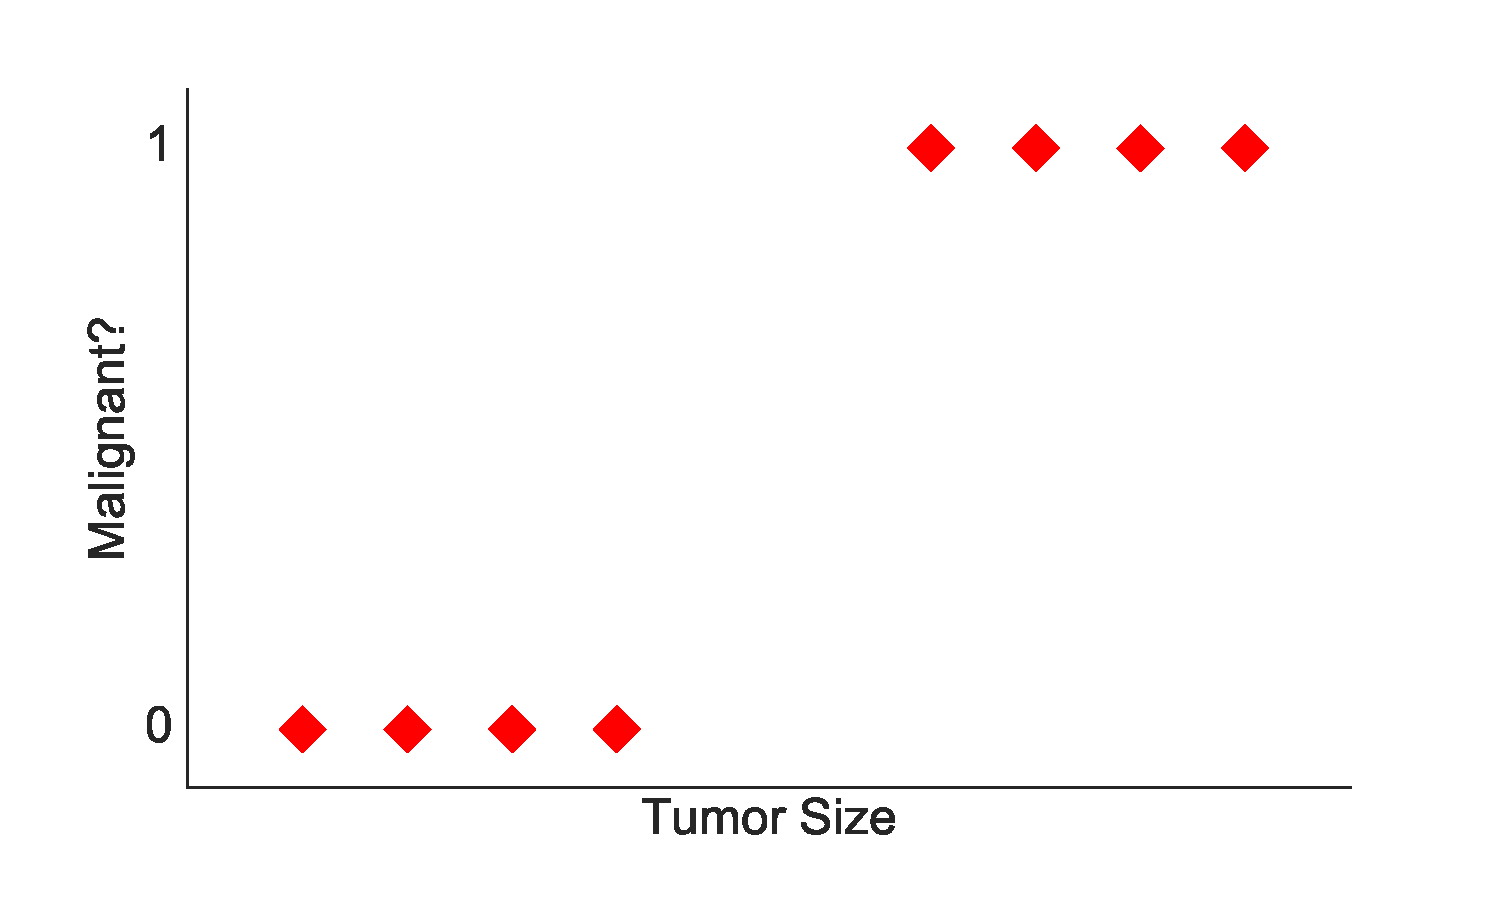
\includegraphics[scale=0.3]{logreg_eg1_maltumor.pdf} 
   		\caption[]{Sample tumor data.}
   		\label{logreg-eg-maltumor-noregline}
	\end{subfigure}
	\begin{subfigure}[t]{0.45\textwidth}
   		\centering
    		\graphicspath{{./Figures/}}
   		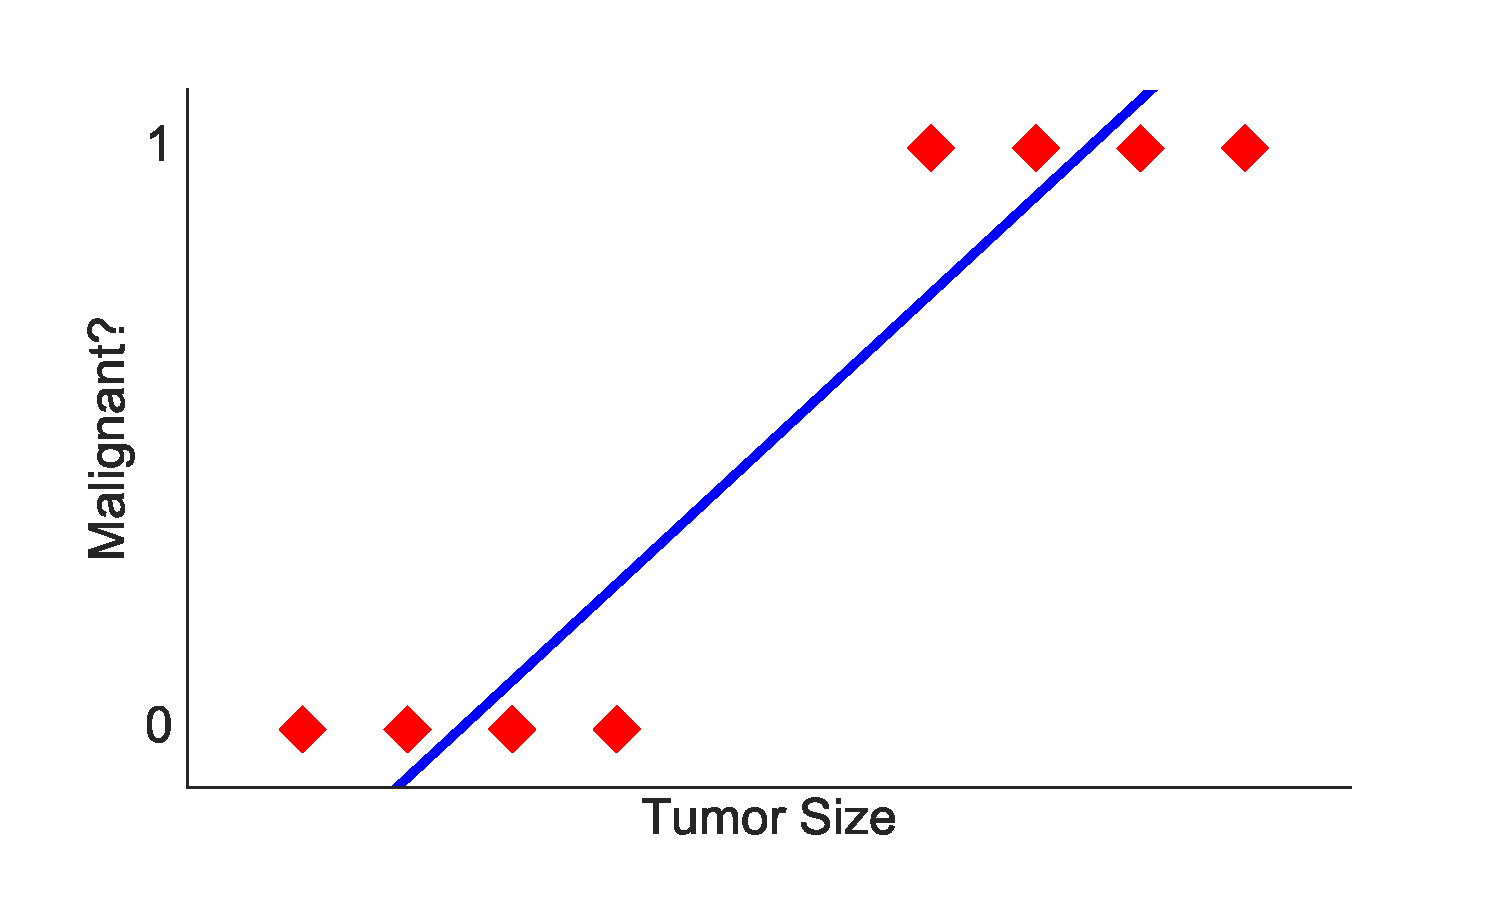
\includegraphics[scale=0.3]{logreg_eg1_maltumor_linreg1.pdf} 
   		\caption[]{Plot of tumors by size with linear regression line $y =  \frac{x-1}{6} - 0.25$.}
   		\label{logreg_eg1_maltumor_linreg1}
	\end{subfigure}
	\caption[]{Plots of tumors by size.}
\end{figure}

To try and make predictions, we can threshold the output at $h_\theta\left( x \right) = 0.5$, and then:
\begin{itemize}
\item If $h_\theta\left(x\right) \geq 0.5$, then predict $y = 1$
\item If $h_\theta\left( x \right) < 0.5$, then predict $y = 0$
\end{itemize}
and you can see this in Figure \ref{logreg_eg1_maltumor_linreg1_threshold.pdf}.

\begin{figure}[h] 
	\centering
	\graphicspath{{./Figures/}} 
	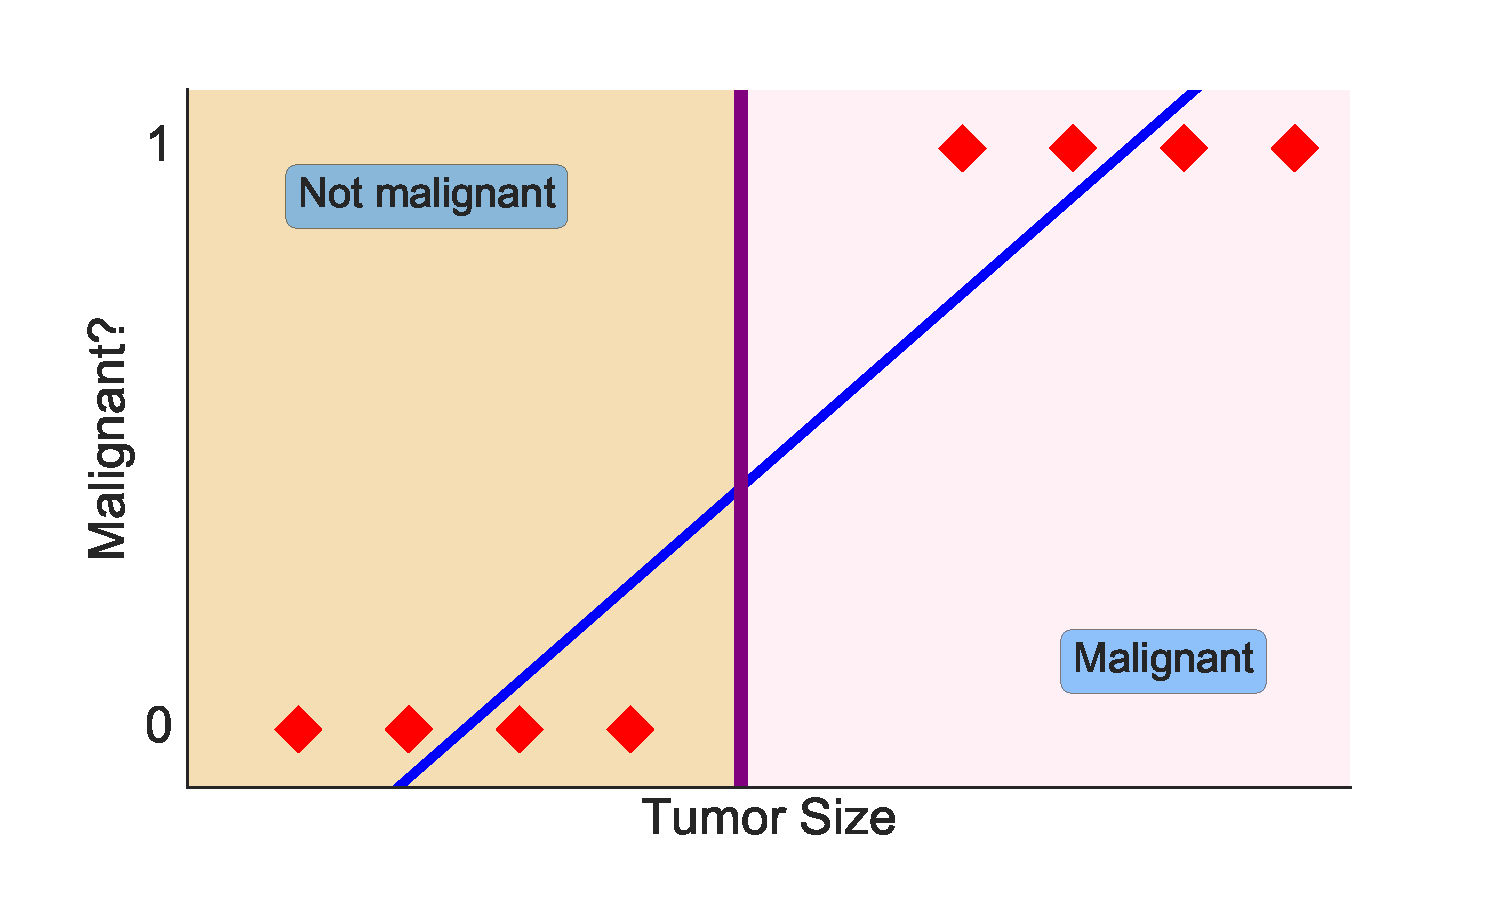
\includegraphics[scale=0.4]{logreg_eg1_maltumor_linreg1_threshold.pdf} 
	\caption[]{Linear regression plotted with classification regions. }
	\label{logreg_eg1_maltumor_linreg1_threshold.pdf}
\end{figure}


In this example, it would seem like linear regression is a good classifier. However, what if we add a new data point for a large tumor. Suddenly, our results look like this

\begin{figure}[h] %  figure placement: here, top, bottom, or page
	\centering
	\graphicspath{{./Figures/}} %Use this to import an image from a subfolder.
	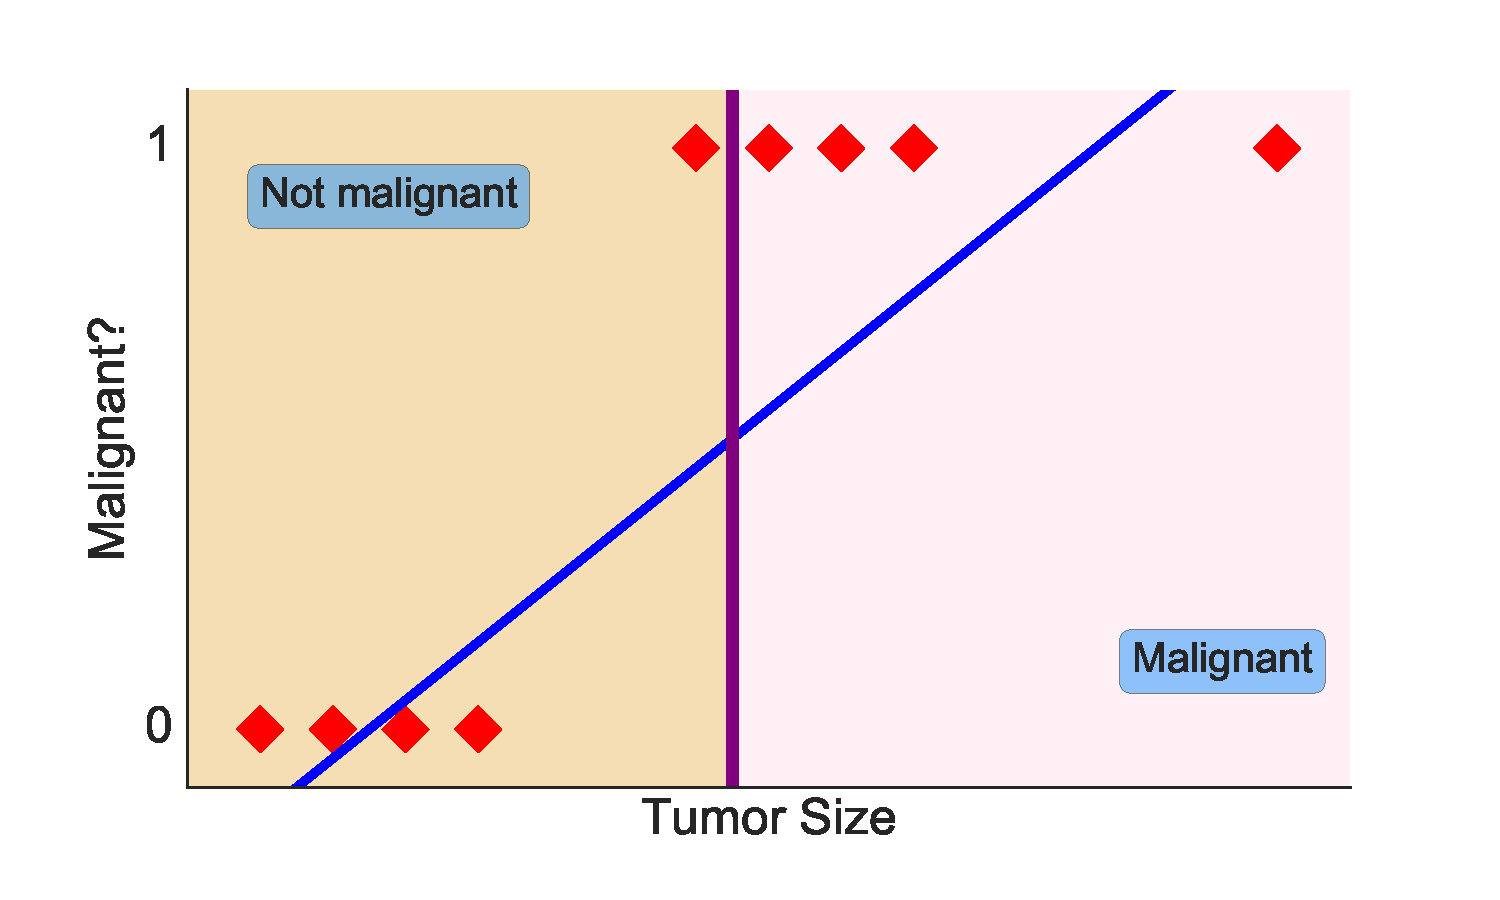
\includegraphics[scale=0.4]{logreg_eg1_maltumor_linreg1_newpoint.pdf} 
	\caption[]{Linear regression plotted with classification regions after a new data point is added. Notice how one of the malignant tumors is now being misclassified as benign.}
	\label{logreg_eg1_maltumor_linreg1_newpoint.pdf}
\end{figure}

and now, we have a malignant tumor being misclassified as benign. Ergo, maybe linear regression isn't the best way to build a binary classifier. 






\section{Hypothesis Representation}
In linear regression, our hypothesis was $h_\theta\left(\vec{x}\right) = \vec{\theta}^\intercal \vec{x}$ For logistic regression, we want our hypothesis to satisfy $0 \leq h_\theta\left(x\right) \leq 1$. To do this, we use the sigmoid function.\footnote{This is also called the logistic function, and is the namesake for logistic regression.} To make this work, we modify our hypothesis to be
\begin{equation}
h_\theta\left(x\right) = g\left(\vec{\theta}^\intercal \vec{x}\right)
\end{equation}
where the function $g\left(z\right)$ is defined as
\begin{equation}
g\left(z\right) = \frac{1}{1 + e^{-z}}
\end{equation}
Thus, to get the hypothesis function using the sigmoid function, just set $z = \vec{\theta}^\intercal \vec{x}$. 

The sigmoid function, shown in Figure \ref{logreg_eg2_sigmoid_func_plot.pdf}, maps any real number onto the interval $\left(0, 1\right)$. This makes it immensely useful for transforming an arbitrary function for use with classification.


\begin{figure}[h] %  figure placement: here, top, bottom, or page
	\centering
	\graphicspath{{./Figures/}} %Use this to import an image from a subfolder.
	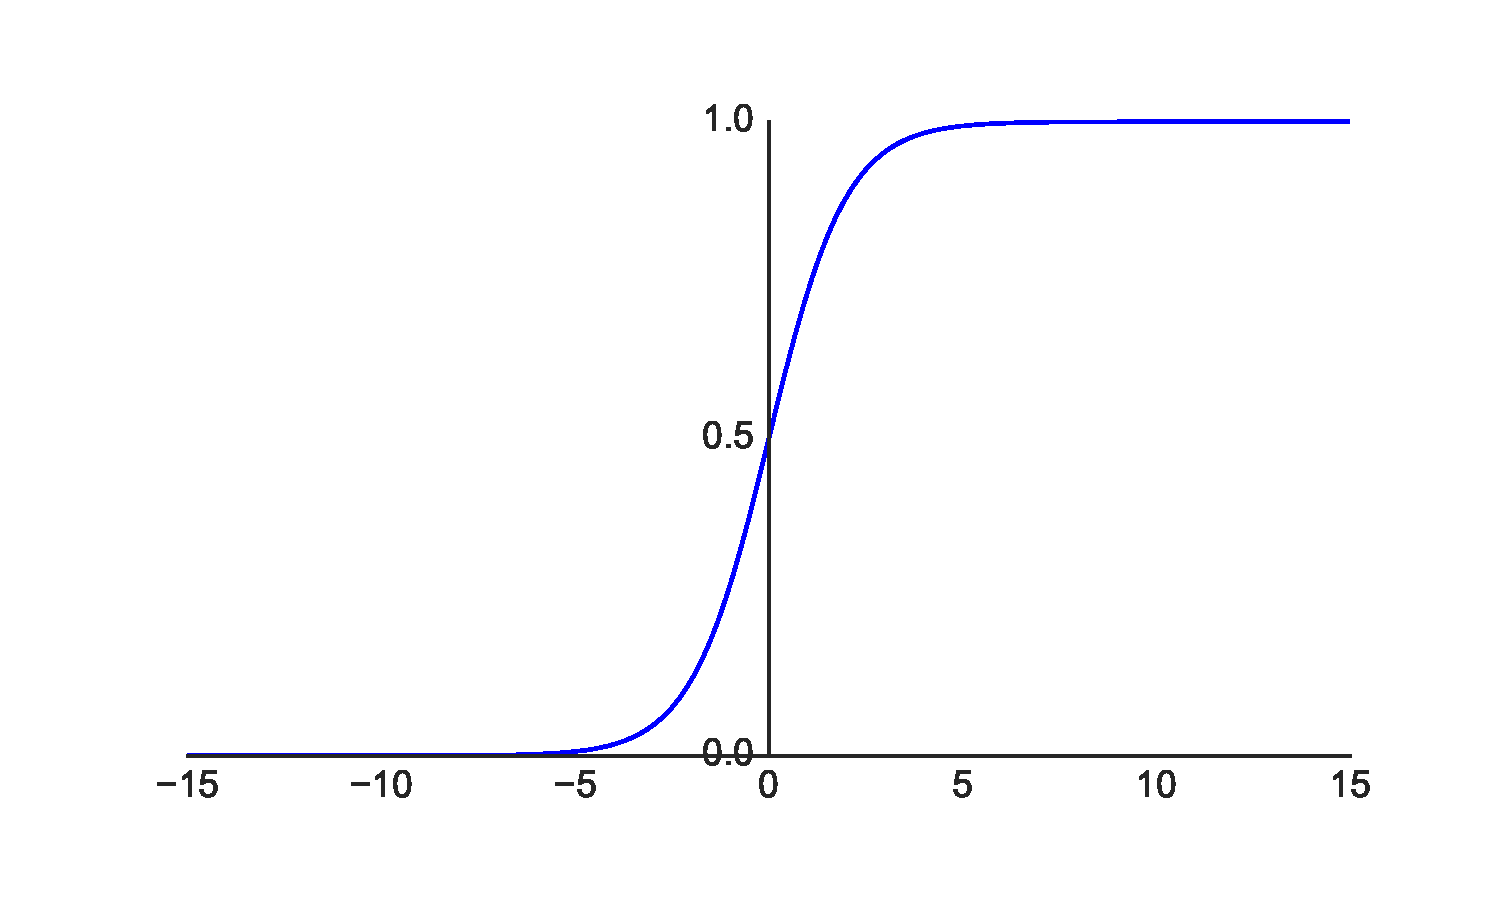
\includegraphics[scale=0.4]{logreg_eg2_sigmoid_func_plot.pdf} 
	\caption[]{Sample plot of the sigmoid function.}
	\label{logreg_eg2_sigmoid_func_plot.pdf}
\end{figure}


\subsection{Interpretation of the Logistic Hypothesis Function}

When examining the hypothesis function output for logistic regression, we interpret $h_\theta\left(x \right)$ is the estimated probability that $y=1$ on an input example $x$. For example, let's revisit the tumor size question from above. We have 
$$
\vec{x} = \left[\begin{array}{c}x_0 \\ x_1 \end{array}\right] = \left[\begin{array}{c}1 \\ \text{tumor size} \end{array}\right]
$$
If our hypothesis $h_\theta\left( x \right) = 0.7$, then we can tell the patient that there is a 70\% chance of the tumor being malignant. 

Slightly more formally, we interpret $h_\theta\left(x\right)$ as:\footnote{This is read as "the probability that $y = 1$, given $x$, parameterized by $\theta$.}
\begin{equation}
h_\theta\left(x\right) = P\left(y=1 | x; \theta\right)
\end{equation}
Thus, by the rules of probability:
\begin{align}
P\left(y=0 | x; \theta\right) + P\left(y=1 | x; \theta\right) = 1 \\
P\left(y=0 | x; \theta\right) = 1 - P\left(y=1 | x; \theta\right)
\end{align}


\subsection{Fitting Logistic Regression to a Binary Classifier}
\label{chaplogreg-sect-hyporeg-subsectbinclasfit}
Now, we need to fit our hypothesis function into a binary classfier: $0$ or $1$. Using our probabilistic interpretation of the logistic hypothesis function, we can make the following supposition:

\begin{align}
y  = 1 &\text{ given that } h_\theta\left(x\right) \geq 0.5 \\
y = 0 &\text{ given that } h_\theta\left(x\right) < 0.5
\end{align}

Recall the plot of the sigmoid function in Figure \ref{logreg_eg2_sigmoid_func_plot.pdf}. We see that $g\left(z\right) \geq 0.5$ when $z \geq 0$. In our case, if we're setting $z = \vec{\theta}^\intercal \vec{x}$, then we have:

\begin{equation}
h_\theta\left(x\right) = g\left(\vec{\theta}^\intercal\vec{x}\right) \geq 0.5 ~~\mbox{ when }~~ \vec{\theta}^\intercal\vec{x} \geq 0
\end{equation}

\noindent From this, we can now state
\begin{align}
\vec{\theta}^\intercal\vec{x} \geq 0 &\implies y = 1 \\
\vec{\theta}^\intercal\vec{x} < 0 &\implies y= 0
\end{align}

\noindent When utilizing the sigmoid function, keep the following in mind:
\begin{itemize}
\item When $z = 0$, then $e^0 = 1$ so $g\left(x\right) = \frac{1}{2}$
\item When $z$ goes to $\infty$, we have $e^{-\infty} \to 0$, and this implies $g\left(x\right) = 1$
\item As $z \to -\infty$, $e^\infty \to \infty \implies g\left(z\right) = 0$
\end{itemize}


\section{Decision Boundary}
\begin{figure}[h] %  figure placement: here, top, bottom, or page
	\centering
	\graphicspath{{./Figures/}} %Use this to import an image from a subfolder.
	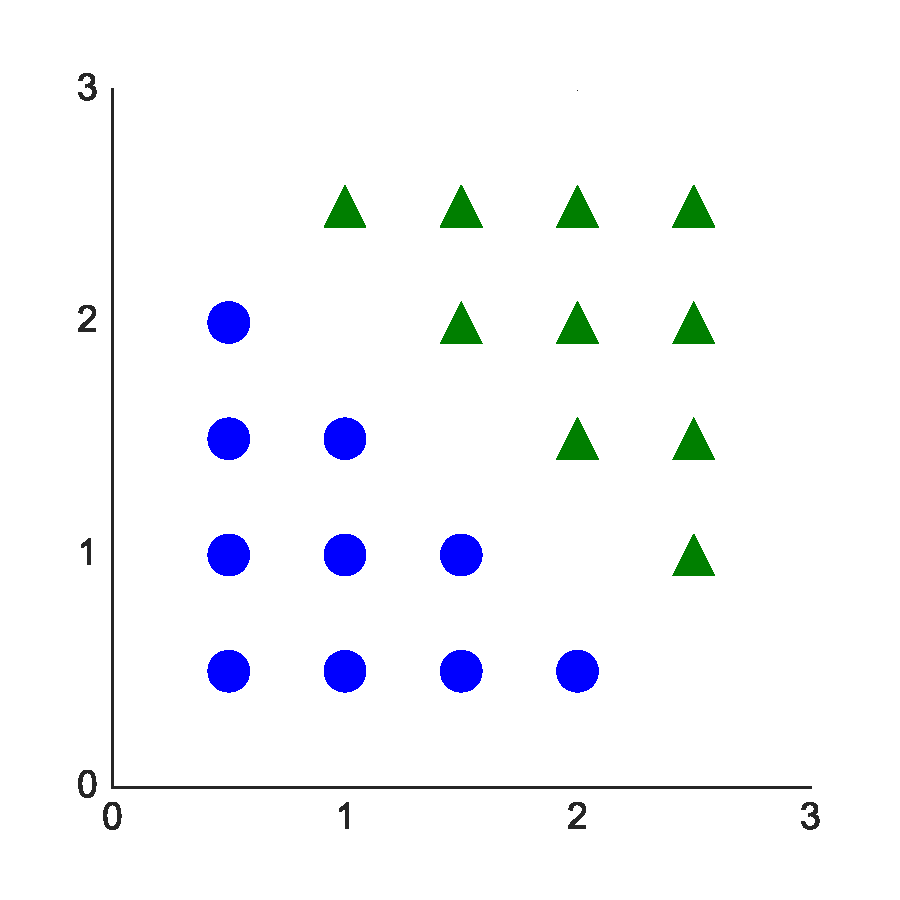
\includegraphics[scale=0.4]{logreg_eg3_decision_bndy_noline.pdf} 
	\caption[]{Sample data.}
	\label{logreg_eg3_decision_bndy_noline.pdf}
\end{figure}

Consider the data plotted in Figure \ref{logreg_eg3_decision_bndy_noline.pdf}. Suppose our hypothesis is given by
$$
h_\theta\left(x\right) = g\left(\theta_0 + \theta_1x_1 + \theta_2x_2\right)
$$
We haven't yet discussed how to fit the parameters of this model (that's coming up next), but suppose we choose the following values for the parameters
$$
\vec{\theta} = \left[\begin{array}{c}\theta_0 \\ \theta_1 \\ \theta_2\end{array}\right] = \left[\begin{array}{c} -3 \\ 1 \\ 1 \end{array}\right]
$$

Given this choice of parameters, let's figure out where $y=1$ and where $y=0$. From \S\ref{chaplogreg-sect-hyporeg-subsectbinclasfit}, recall that we predict $y=1$ when $\vec{\theta}^\intercal\vec{x} \geq 0$, so here, we predict $y=1$ if $-3 + x_1 + x_2 \geq 0$. If we solve this for $x_1 + x_2$ we get
$$
x_1 + x_2 \geq 3 \implies y = 1
$$
If we change this to a pure equality, $x_1 + x_2 = 3$, we have the equation of a straight line (shown on Figure \ref{logreg_eg3_decision_bndy_withline.pdf}). The line drawn, is called the \textbf{decision boundary}. The decision boundary is the line created by the hypothesis function that separates the area where we classify $y=0$ and where $y=1$.

\begin{figure}[h] %  figure placement: here, top, bottom, or page
	\centering
	\graphicspath{{./Figures/}} %Use this to import an image from a subfolder.
	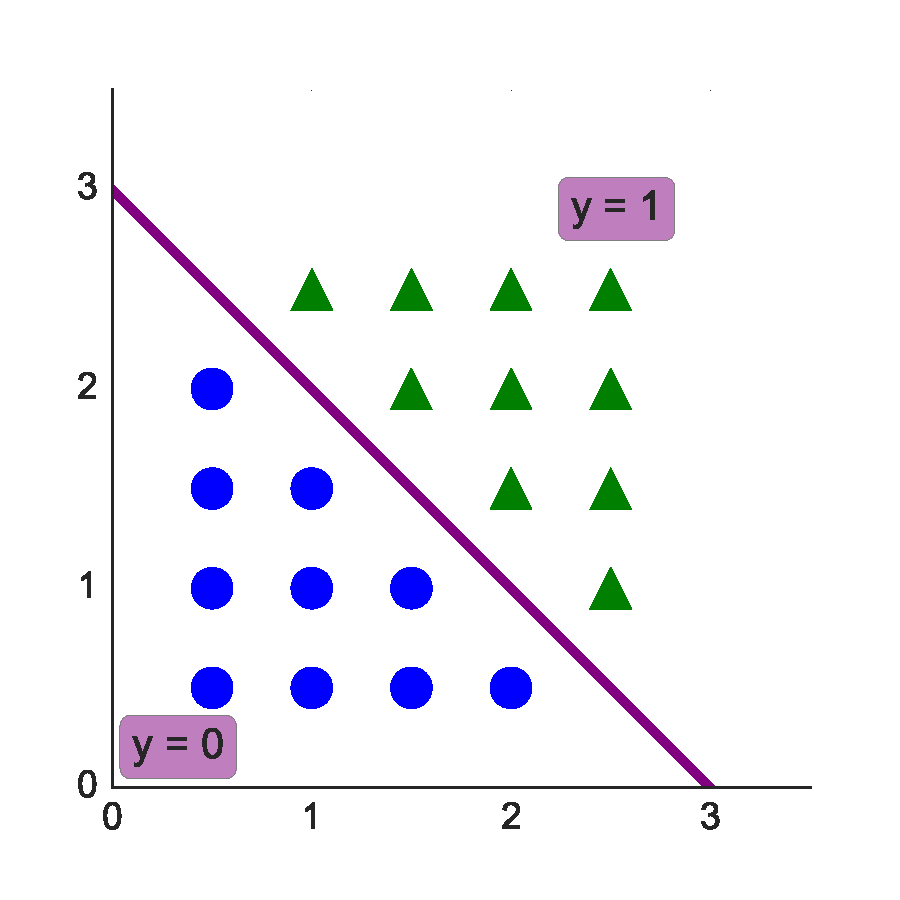
\includegraphics[scale=0.4]{logreg_eg3_decision_bndy_withline.pdf} 
	\caption[]{Sample data with plotted decision boundary.}
	\label{logreg_eg3_decision_bndy_withline.pdf}
\end{figure}

To be clean, the decision boundary is a property of the hypothesis function, and not a property of the dataset. We fit the parameters of the hypothesis based on the training data, but once those parameters are set, the decision boundary is a property solely of the hypothesis function. 

Now, suppose we have data as shown below in Figure \ref{logreg_eg3_decision_bndy_nonlinear_nocirc.pdf}. It's fairly obvious that no straight line decision boundary will work for this data. Again, we don't know how to fit the parameters for this model yet, but say our hypothesis function looks like this
$$
h_\theta\left(x\right) = g\left(\theta_0 + \theta_1x_1 + \theta_2x_2 + \theta_3x_1^2 + \theta_4x_2^2\right)
$$
Imagine we fit the parameters appropriately, and we get
$$
\vec{\theta} = \left[\begin{array}{c} \theta_0 \\ \theta_1 \\ \theta_2 \\ \theta_3 \\ \theta_4 \end{array}\right] = \left[\begin{array}{c}-1 \\ 0 \\ 0 \\ 1 \\ 1 \end{array}\right]
$$
Then, our hypothesis predicts that $y=1$ when $x_1^2 + x_2^2 \geq 1$. This is the equation for a circle of radius $1$, centered at the origin (see Figure \ref{logreg_eg3_decision_bndy_nonlinear.pdf}).
\begin{figure}[h]
	\centering
	\begin{subfigure}[t]{0.45\textwidth}
   		\centering
    		\graphicspath{{./Figures/}}
  		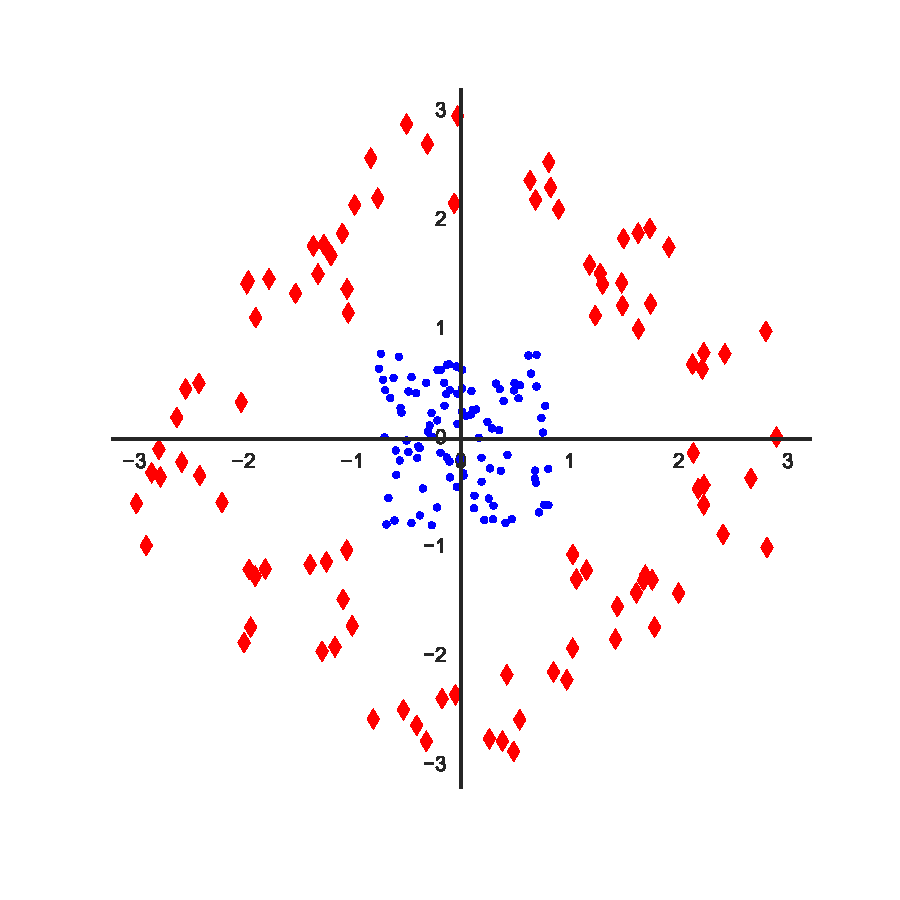
\includegraphics[scale=0.4]{logreg_eg3_decision_bndy_nonlinear_nocirc.pdf} 
   		\caption[]{This is a sample of data with no clear linear decision boundary.}
   		\label{logreg_eg3_decision_bndy_nonlinear_nocirc.pdf}
	\end{subfigure}
	\begin{subfigure}[t]{0.45\textwidth}
   		\centering
    		\graphicspath{{./Figures/}}
   		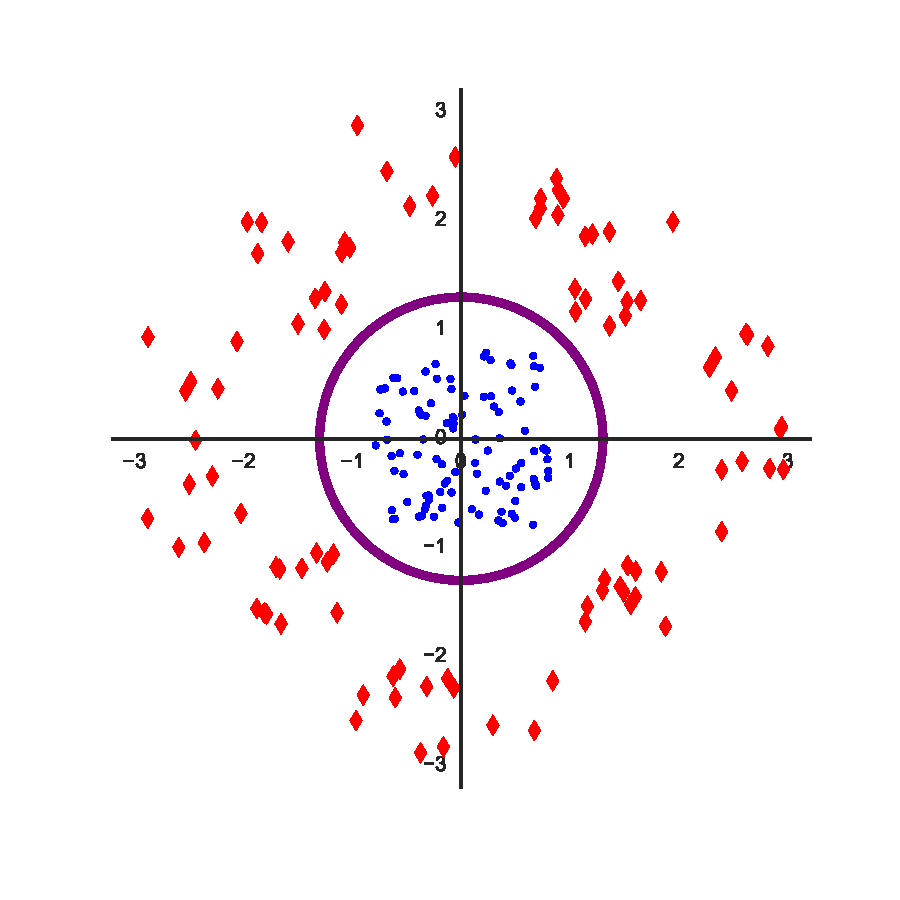
\includegraphics[scale=0.4]{logreg_eg3_decision_bndy_nonlinear.pdf} 
   		\caption[]{By altering our hypothesis function to include polynomial terms, we can have a non-linear decision boundary.}
   		\label{logreg_eg3_decision_bndy_nonlinear.pdf}
	\end{subfigure}
	\caption[]{Data that can't be fit with a linear decision line.}
\end{figure}
In this case, we predict $y=1$ everywhere outside the purple circle, and $y=0$ everywhere inside the circle. 

With even higher order polynomials, we can get even more complicated decision boundaries. 


\section{Cost Function}
Imagine we have a training set of data with $m$ examples
$$
\left\{ \left(x^{\left(1\right)}, y^{\left(1\right)}\right), \left(x^{\left(2\right)}, y^{\left(2\right)}\right), \cdots, \left(x^{\left(m\right)}, y^{\left(m\right)}\right) \right\}
$$
and $n$ features, represented by an $n+1$-dimensional feature vector
$$
x \in \left[\begin{array}{c} x_0 \\ x_1 \\ \vdots \\ x_n \end{array}\right]
$$
where $x_0 = 1$ and our output $y \in \{0, 1\}$. Our hypothesis is given by
\begin{equation}
h_\theta\left(x\right) = \frac{1}{1 + e^{-\theta^{{}^\intercal}x}}
\end{equation}
How do we choose the parameters for this model? For linear regression, we had the following cost function (adjusted slightly, we moved the $\tfrac{1}{2}$ to the inside of the summation)
\begin{equation}
J\left(\theta\right) = \frac{1}{m} \sum_{i=1}^m \frac{1}{2} \left(		h_\theta\left(x^{\left(i\right)}\right) - y^{\left(i\right)}	\right)^2
\end{equation}
but we're going to change how we write this function a little bit. Instead, we'll write
\begin{equation}
J\left(\theta\right) = \frac{1}{m} \sum_{i=1}^m \text{cost}\left(	h_\theta\left(x^{\left(i\right)}\right), y^{\left(i\right)}\right)
\end{equation}
where we'll define the cost function to be
\begin{equation}
\text{cost}\left(	h_\theta\left(x^{\left(i\right)}\right), y^{\left(i\right)}\right) = \frac{1}{2} \left(h_\theta\left(x^{\left(i\right)}\right) - y^{\left(i\right)}	\right)^2
\end{equation}
This allows us to see more clearly that the cost function is really the sum over the cost term. To simplify even further, we'll remove the superscripts $\left(i\right)$
\begin{equation}
\text{cost}\left(h_\theta\left(x\right), y\right) = \frac{1}{2} \left(	h_\theta\left(x\right) - y \right)^2
\end{equation}


If we try an minimize this cost function, this turns out to be a non-convex function. That means that the may be several local minima, which would prevent our gradient descent algorithm from working well. You can see a sample non-convex function in Figure \ref{logreg_eg4_sample_nonconvex_curve.pdf}. What we want instead, is a convex function (like a parabola) that only has a single minimum that is the global minimum. The sigmoid function is a non-linear signal function, so $J\left(\theta\right)$ ends up being non-convex. 
\begin{figure}[h] %  figure placement: here, top, bottom, or page
	\centering
	\graphicspath{{./Figures/}} %Use this to import an image from a subfolder.
	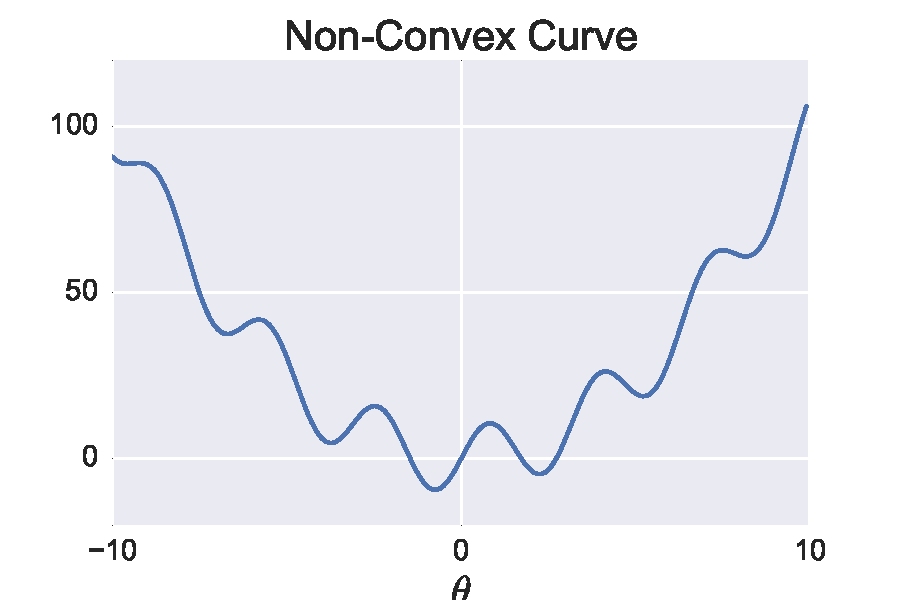
\includegraphics[scale=0.6]{logreg_eg4_sample_nonconvex_curve.pdf} 
	\caption[]{A non-convex curve. Notice all of the local minima.}
	\label{logreg_eg4_sample_nonconvex_curve.pdf}
\end{figure}

We need to define a new (convex) cost function that will allow us to determine the parameters in our hypothesis. For logistic regression, we use the following cost function
\begin{equation}
\text{cost}\left(h_\theta\left(x\right), y\right) = \begin{cases} -\log\left(h_\theta\left(x\right)\right) & \text{if } y = 1 \\ -\log\left(1 - h_\theta\left(x\right)\right) &\text{if } y = 0 \end{cases}
\end{equation}
We plot this cost function below in Figure \ref{chaplogreg-sectcostfunct-plotcostfuncsample}. 

\begin{figure}[h]
	\centering
	\begin{subfigure}[t]{0.45\textwidth}
   		\centering
    		\graphicspath{{./Figures/}}
  		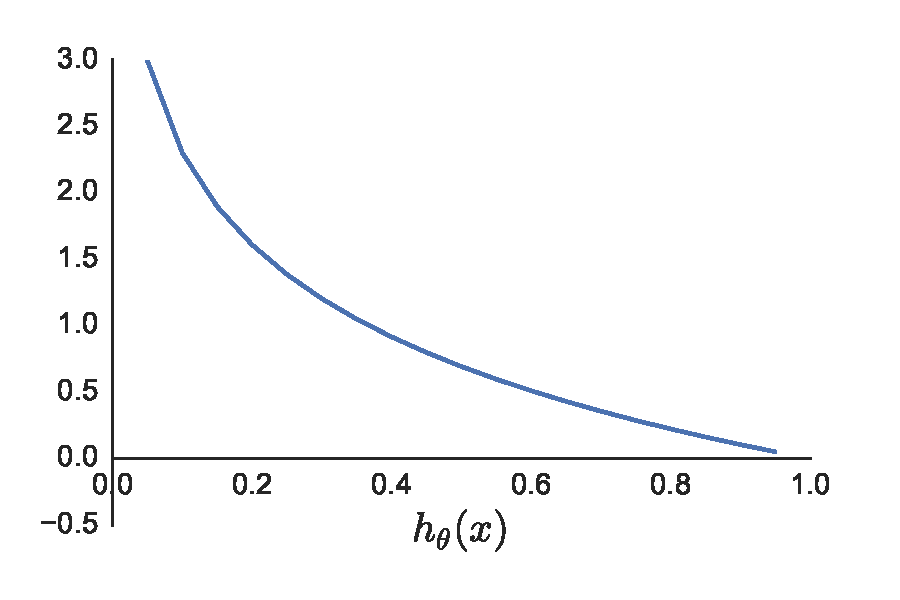
\includegraphics[scale=0.5]{logreg_eg5_cost_func_y1.pdf} 
   		\caption[]{$y=1$.}
   		\label{logreg_eg5_cost_func_y1.pdf}
	\end{subfigure}
	\begin{subfigure}[t]{0.45\textwidth}
   		\centering
    		\graphicspath{{./Figures/}}
   		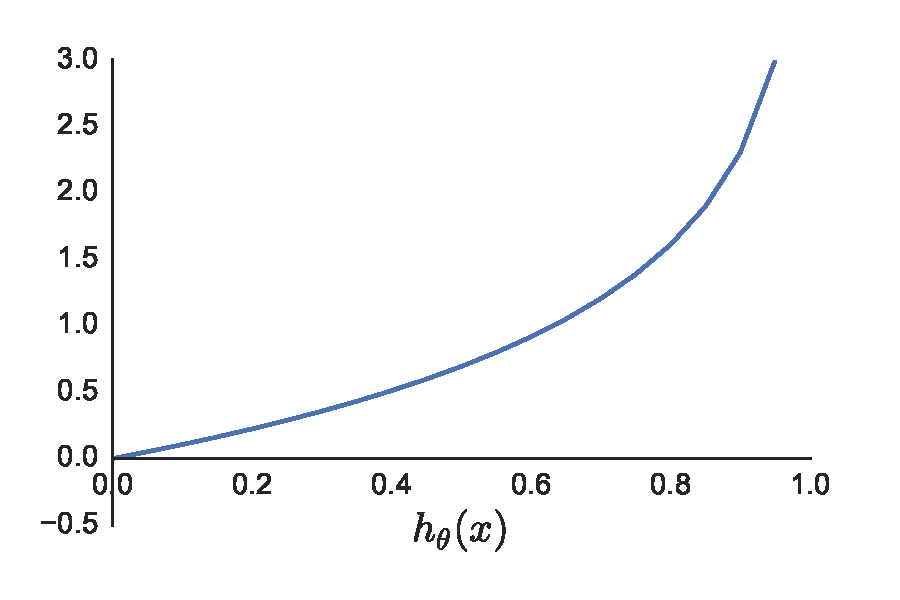
\includegraphics[scale=0.5]{logreg_eg5_cost_func_y0.pdf} 
   		\caption[]{$y=0$}
   		\label{logreg_eg5_cost_func_y0.pdf}
	\end{subfigure}
	\caption[]{The piecewise cost function for logistic regression. }
	\label{chaplogreg-sectcostfunct-plotcostfuncsample}
\end{figure}

The shape of the curve comes from standard plot of $\log\left(x\right)$, and we just use a negative to flip it upside-down. This cost function, has some very desirable properties for us right now. 


\noindent \begin{minipage}{\linewidth}
\begin{itemize}
\item If $y = 1$, then $h_\theta\left(x\right) = 1$ and the cost is zero. However, as $h_\theta\left(x\right) \to 0$ then $\text{cost} \to \infty$. This captures the intuition that if $h_\theta\left(x\right) = 0$, but $y=1$, we'll penalize the learning algorithm by a very large cost. 
\item For $y=0$, this is reversed. If we have $y=0$ and $h_\theta\left(x\right) = 0$, then the cost is $0$. If $y=0$, the cost grows very large as $h_\theta\left(x\right)$ increases towards $1$. 
\end{itemize}
\end{minipage}



































